\documentclass[aspectratio=169,11pt]{beamer}
\usepackage[T1]{fontenc}
\usepackage{lmodern}
\usepackage{graphicx}
\usepackage{booktabs}
\newcommand{\TitleMain}{Method for Walk Correction using Leading Edge Slope:}
\newcommand{\TitleSub}{Derived from dual threshold feature of TOFHIR2C}
\newcommand{\ShortTitle}{Leading-edge slope and walk correction}

% Generated from frozen numerical results by build_assets.py.
\newcommand{\TimingCount}{10127}
\newcommand{\DBefore}{55.16}
\newcommand{\DAfter}{54.82}
\newcommand{\DLow}{54.32}
\newcommand{\DHigh}{55.22}
\newcommand{\DSD}{61.26}
\newcommand{\DTail}{1.57}
\newcommand{\RBefore}{77.69}
\newcommand{\RAfter}{64.16}
\newcommand{\RLow}{63.27}
\newcommand{\RHigh}{64.99}
\newcommand{\RSD}{70.33}
\newcommand{\RTail}{1.56}
\newcommand{\RefBinsA}{19}
\newcommand{\RefBinsB}{19}
\newcommand{\RefBinsC}{20}
\newcommand{\RefBinsD}{19}
\newcommand{\ExampleAWC}{18.332}
\newcommand{\ExampleLow}{18.120}
\newcommand{\ExampleHigh}{18.607}
\newcommand{\ExampleRMS}{6.80}
\newcommand{\GapCount}{703}
\newcommand{\SummaryChi}{538.6}
\newcommand{\PredictorRMSE}{3.22}
\newcommand{\PredictorFraction}{14.1}

\usetheme{default}
\setbeamercolor{normal text}{fg=black,bg=white}
\setbeamercolor{structure}{fg=black}
\setbeamersize{text margin left=7mm,text margin right=7mm}
\setbeamertemplate{navigation symbols}{}
\setbeamerfont{frametitle}{size=\large,series=\bfseries}
\setbeamertemplate{headline}{%
  \hbox to \paperwidth{\hspace{7mm}\scriptsize\color{black!55}Internal review draft -- 22 October 2026
  \hfill\raisebox{0pt}[9mm][1mm]{
\includegraphics[height=7mm]{CMSlogo_black_label_1024.png}}\hspace{6mm}}}
\setbeamertemplate{footline}{%
  \hbox to \paperwidth{\hspace{7mm}\scriptsize\ShortTitle
  \hfill V2 slides -- draft 1\quad\insertframenumber/\inserttotalframenumber\hspace{7mm}}\vspace{2mm}}
\setbeamertemplate{frametitle}{\vspace{-1mm}\insertframetitle\par\vspace{1mm}}
\setlength{\parskip}{4pt}
\newcommand{\Code}[2]{\href{https://github.com/De-Cristo/LecroyTranslator4CMSTimingDetector/blob/45a907c422d6c8afbe0cdf44cd2827d3433d0f97/#1}{#2}}
\newcommand{\Source}[1]{\par\smallskip{\fontsize{8}{9.5}\selectfont\color{black!65}#1\par}}
\newcommand{\PlotSlide}[4]{%
  \begin{frame}[t]{#1}
  \begin{columns}[T,onlytextwidth]
    \begin{column}{.63\textwidth}
      \centering\includegraphics[width=\linewidth,height=51mm,keepaspectratio]{figures/#2.pdf}
    \end{column}
    \begin{column}{.35\textwidth}\fontsize{10}{12}\selectfont #3\end{column}
  \end{columns}
  \Source{#4}
  \end{frame}}
\newcommand{\TitleSlide}{%
  \begin{frame}
    \centering{\Large\TitleMain\par}\vspace{3mm}
    {\large\TitleSub\par}\vspace{8mm}
    {\large CMS\par}\vspace{2mm}
    \href{mailto:cms-dpg-conveners-mtd@cern.ch}{cms-dpg-conveners-mtd@cern.ch}
    \vspace{7mm}\par{\small Discussion draft; not approved for public release.}
  \end{frame}}
\hypersetup{pdftitle={\TitleMain\space\TitleSub},pdfauthor={CMS}}

\begin{document}
\TitleSlide

\begin{frame}{Purpose: rapid, repeatable walk calibration at HL-LHC}
\large
BTL needs frequent recalibration as detector response evolves.
For about 330\,000 channels, a consistent physical parametrization matters.
\medskip

\textbf{Goal:} predict each channel's walk correction from simple internal
charge and dual-threshold measurements, without a dedicated $t_0$ reference
for every calibration.
\medskip

\normalsize
TOFHIR2C measures the leading-edge slope. This gives a common correction
form and internal observables with which to predict its amplitude, AWC.
The MCP study benchmarks this approach; transfer to new data and operating
conditions is the next test.
\Source{BTL and TOFHIR2C: Refs.~\cite{MTDTDR,TOFHIR2}; dual-threshold motivation and bench study: Ref.~\cite{DualThreshold}.}
\end{frame}

\begin{frame}{Charge-based calibration works, but its coefficients vary}
\normalsize
The MCP reference note obtains good walk descriptions with a quadratic in
inverse charge~\cite{ReferenceNote}:
\[
W_i(Q)=a_i+b_i/Q+c_i/Q^2.
\]
\centering
\small
\begin{tabular}{rrrrr}
\toprule
Bar & Channel & $a_i$ [ns] & $b_i$ [ns ADC] & $c_i$ [ns ADC$^2$]\\
\midrule
7 & 133 & 0.0796 & 238.3 & $-2.156\times10^4$\\
7 & 154 & $-0.5155$ & 422.6 & $-5.583\times10^4$\\
8 & 137 & 0.1218 & 198.5 & $-1.523\times10^4$\\
8 & 150 & $-0.2292$ & 388.9 & $-5.132\times10^4$\\
\bottomrule
\end{tabular}
\par\raggedright
\normalsize
The shape coefficients vary substantially even among four channels.
Use pulse slope to seek a more consistent physical description.
\Source{Original reference coefficients, also reproduced in Table 1 of the detector note.
$Q$ is the ADC charge proxy; $a_i$ includes an arbitrary timing offset.
Coefficient variation alone is not a measure of calibration precision.}
\end{frame}

\begin{frame}{TOFHIR2C measures the leading-edge slope with two thresholds}
\normalsize
Larger pulses cross a fixed threshold earlier: the timestamp depends on amplitude.
Two thresholds also measure how fast the pulse rises~\cite{TOFHIR2,DualThreshold}.
\[
I_1<I_2,\qquad t_1<t_2,\qquad
S=\frac{I_2-I_1}{t_2-t_1}\quad[\mu\mathrm{A/ns}].
\]
Locally, an approximately linear leading edge gives
\[
\Delta t\simeq\frac{\Delta I}{S}.
\]
\textbf{Physical model:} describe amplitude walk with an inverse slope,
rather than an independent polynomial shape for every channel.
\Source{$S$ is a finite-interval slope proxy, not the instantaneous derivative.
Run 4076 uses $\Delta I=7.8125\,\mu$A from the implemented threshold conversion.
The fitted AWC need not equal this threshold separation.
\Code{Q_Walk/qwalk_core.py}{GitHub: timing and threshold reconstruction}.}
\end{frame}

\PlotSlide{Measure the charge-to-slope mapping using internal hits}{slope_ch137}{
Select both ends of one bar; leave the other module unconstrained.

Use physical threshold crossings and the peak-right charge region.

Fit ten profile means with SEM weights:
\[
\overline S_i(Q)=c_{0,i}+c_{1,i}Q.
\]
No MCP time enters this fit.
}{Channel 137, run 4076: 19\,126 selected hits. Points are mean slopes; bars show hit SD, not uncertainty on the mean.
The band is the conditional 68\% interval from 1000 hit-bootstrap refits with fixed bins.
The profile averages the noisy single-hit slope measurements.}

\begin{frame}{One amplitude describes walk once the slope is calibrated}
\large
\[
W_i(Q)=\frac{A_i}{c_{0,i}+c_{1,i}Q},\qquad
t_{\rm corr}=t_{\rm measured}-W_i(Q).
\]
\normalsize
\begin{itemize}
\item Internal hits determine $c_{0,i}$ and $c_{1,i}$, the charge-to-slope mapping.
\item One amplitude $A_i$ (AWC, in $\mu$A) then sets the walk magnitude.
\item AWC is constant per channel and configuration; the correction varies with $Q$.
\item Channel timing offsets are a separate calibration.
\end{itemize}
\medskip
\textbf{The remaining task is to predict AWC from internal observables.}
Use the MCP-calibrated channels to develop and test that prediction.
\Source{Apply the model within its calibrated charge range, with $c_{0,i}+c_{1,i}Q>0$.
The slope fit alone does not fix AWC. The common functional form follows the dual-threshold model in Ref.~\cite{DualThreshold}.}
\end{frame}

\begin{frame}[t]{The single-amplitude model closely follows the MCP curves}
\begin{columns}[T,onlytextwidth]
\begin{column}{.49\textwidth}
\centering\textbf{Channel 137}\par
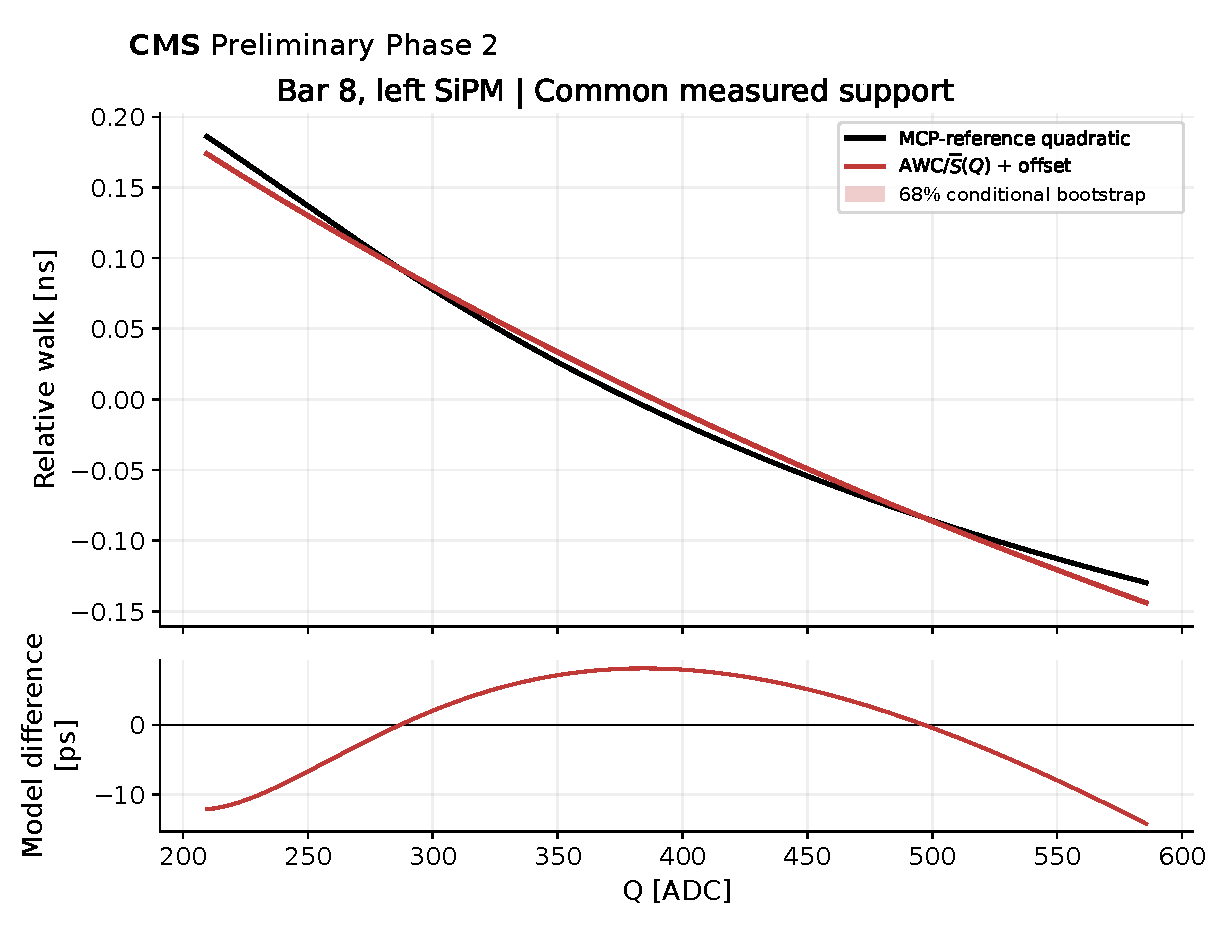
\includegraphics[width=\linewidth,height=43mm,keepaspectratio]{figures/comparison_ch137.pdf}
\end{column}
\begin{column}{.49\textwidth}
\centering\textbf{Channel 154}\par
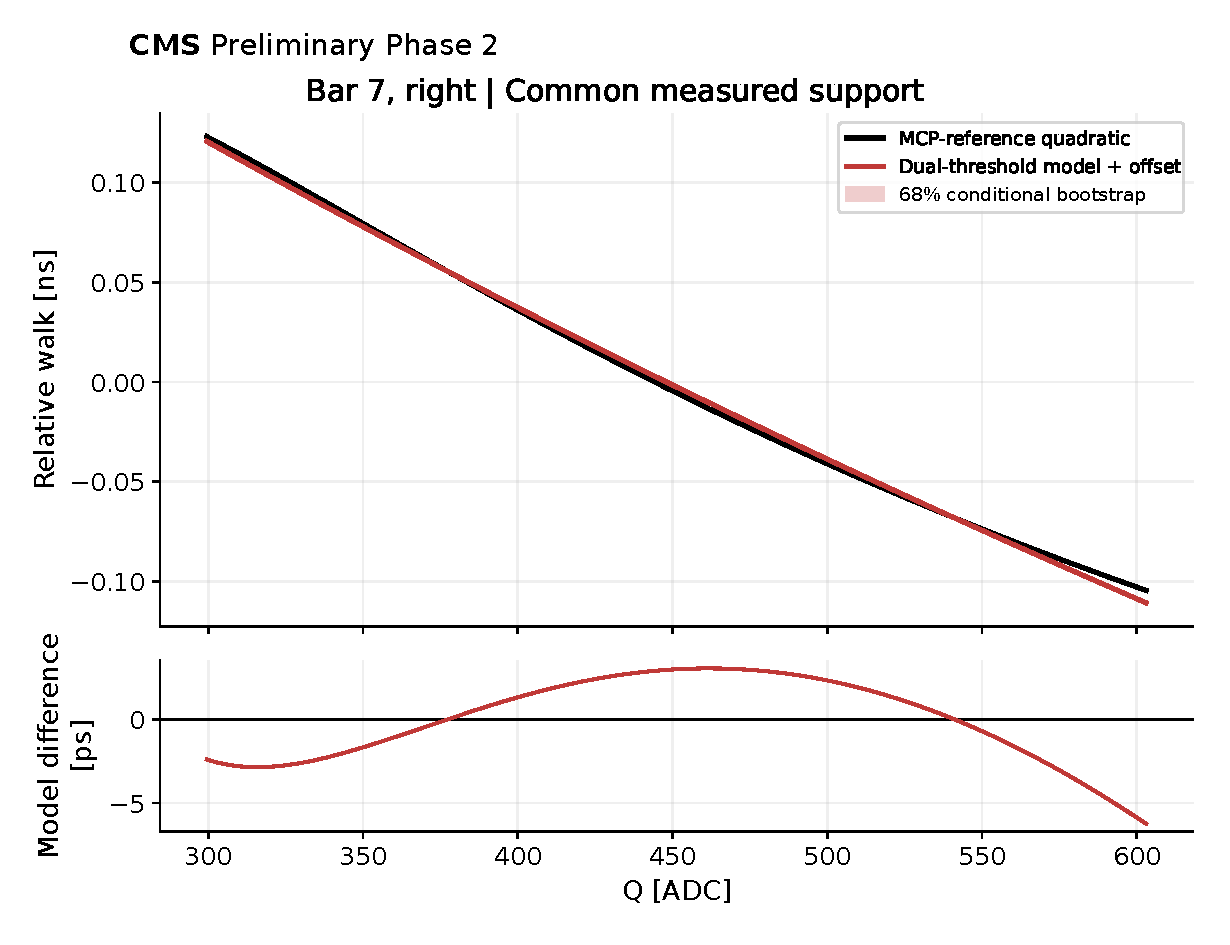
\includegraphics[width=\linewidth,height=43mm,keepaspectratio]{figures/comparison_ch154.pdf}
\end{column}
\end{columns}
\Source{Black: MCP quadratic (run 4399); red: inverse-slope model (run 4076).
AWC and an offset are fitted over charge intervals populated in both runs, which contain different events.
Channel 137 has \ExampleRMS\,ps RMS curve mismatch. Lower panels show curve differences, not event resolution.
Bands propagate slope-fit statistics with the MCP curve fixed. This tests the functional form, before predicting AWC.}
\end{frame}

\begin{frame}{Toward calibration from internal data alone}
\normalsize
\begin{enumerate}
\item Accumulate internal hits and fit $\overline S_i(Q)=c_{0,i}+c_{1,i}Q$.
\item Use the slope coefficients and charge spectrum to predict one AWC per channel.
\item Construct $W_i(Q)=A_i/\overline S_i(Q)$ and correct each timestamp.
\end{enumerate}
\medskip
\textbf{Present evidence:} internal observables carry information about AWC.
An exploratory model tested on excluded bars gives a \PredictorFraction\% RMS
fractional prediction error in ten selected channels (backup).
\medskip

\textbf{Next:} freeze the predictor and test additional channels, independent
runs and operating conditions; assess the corrected timing resolution.
Cosmic-ray data are a possible calibration source to investigate.
\Source{Model development uses MCP-derived AWC targets. Once trained, prediction inputs are internal;
portability of the learned relation is not yet established. The current test is not a universal precision guarantee.}
\end{frame}

\begin{frame}[t]{Final result: internal slope information constrains AWC}
\centering
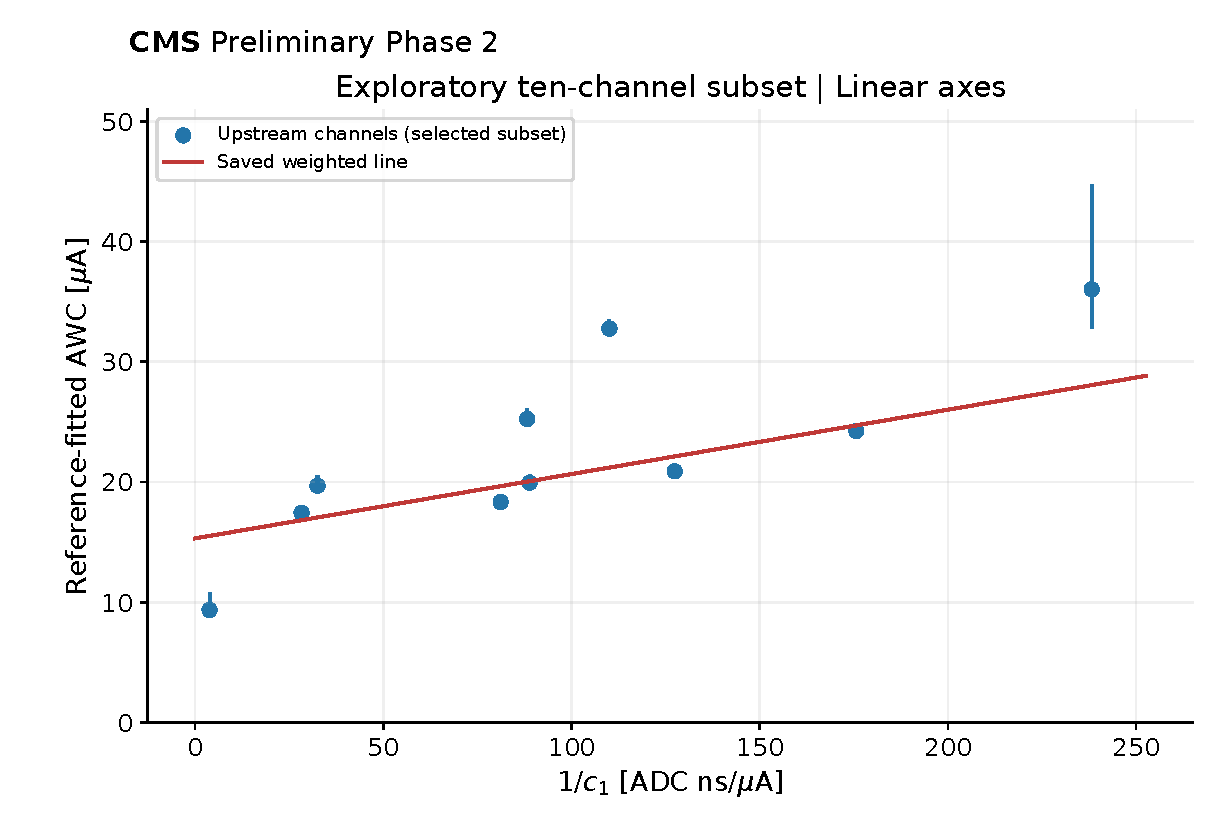
\includegraphics[width=\linewidth,height=48mm,keepaspectratio]{figures/awc_summary_selected.pdf}
\par\raggedright
\Source{The final observable of the original detector note: AWC versus $1/c_1$, the inverse slope-to-charge coefficient.
Each point is one channel, not a charge bin. AWC is benchmarked against MCP; $c_1$ uses internal hits.
The ten-channel trend motivates prediction, but the line is not a precision calibration ($\chi^2/\mathrm{ndf}=\SummaryChi/8$).
Bars: slope-only 16--84\% bootstrap intervals; reference errors and correlations are omitted. More independent data are needed.}
\end{frame}

\PlotSlide{Backup: a physics-motivated predictor tested on excluded bars}{internal_predictor}{
Assume a shared local derivative $K\simeq-dW/d\ln Q$ at $Q_*$:
\[
A_i=K\,\frac{\overline S_i(Q_*)^2}{c_{1,i}Q_*}.
\]
$Q_*$: selected-charge median per channel.

Learn $K$ from other bars; predict the excluded bar.

RMS error: \PredictorRMSE\,$\mu$A; fractional RMS: \PredictorFraction\%.
}{Ten upstream channels, six held-out bars. Learn $K$ from other bars' MCP-calibrated AWC; predict with internal observables.
Horizontal bars: reference-AWC intervals, not prediction errors. Input--target correlations and full prediction uncertainties are unpropagated;
transfer needs independent tests.}
% Original bibliography, condensed to one slide without changing entries.
\begin{frame}[t]{References}
\fontsize{7}{8}\selectfont
\setlength{\parskip}{0pt}
\setbeamertemplate{bibliography item}[text]
\begin{columns}[T,onlytextwidth]
\begin{column}{.485\textwidth}
\begin{thebibliography}{12}
\setlength{\itemsep}{1pt}
\setlength{\parsep}{0pt}
\bibitem[1]{ALICEPerformance}
``Performance of the ALICE Time-Of-Flight detector at the LHC'',
Eur. Phys. J. Plus (2013) 128: 44
\bibitem[2]{ALICEPID}
``PID performance of the ALICE-TOF detector at Run 2'', N. Jacazio in
Proceedings of LHCP2018, \url{https://pos.sissa.it/321/232/}.
\bibitem[3]{MTDTDR}
CMS Collaboration, ``A MIP Timing Detector for the CMS Phase-2 Upgrade''.
Technical Report CERN-LHCC-2019-003. CMS-TDR-020, CERN, Geneva, 2019 and
``A High-Granularity Timing Detector for the ATLAS Phase-II Upgrade'',
CERN-LHCC-2020-007; ATLAS-TDR-031
\bibitem[4]{Leo}
W. R. Leo, ``Techniques For Nuclear and Particle Physics Experiments'',
p.326, Springer-Verlag Berlin Heidelberg.
\bibitem[5]{DualThreshold}
S. White and A. Boletti, ``Amplitude Walk in Fast Timing: The Role of Dual Thresholds''
2026 JINST V21 P02001.
\bibitem[6]{ReferenceNote}
S. White and Licheng J. Zhang, ``September 2025 BTL Testbeam Reference Bar Walk
Calibration from Hamamatsu MCP-PMT '',cms note.
\end{thebibliography}
\end{column}
\begin{column}{.485\textwidth}
\begin{thebibliography}{12}
\setlength{\itemsep}{1pt}
\setlength{\parsep}{0pt}
\bibitem[7]{TOFHIR2}
E. Albuquerque et al., ``TOFHIR2: The readout ASIC of the CMS Barrel MIP Timing
Detector'', arxiv:2404.01208
\bibitem[8]{Grund}
J.E. Grund, SLAC-PUB-2416 (Oct. 1979).
\bibitem[9]{Frolov}
A.R. Frolov, T.V. Oslopova, Yu.N. Pestov, ``Double threshold discriminator for
timing measurements'', Nuclear Instruments and Methods Volume 356, Issues 2/3
(1995) \url{https://doi.org/10.1016/0168-9002(94)01239-3}.
\bibitem[10]{LGAD}
This will arise in LGAD that are not thinned to remove the effect (J. Vavra,
private communication). See also PICOSEC, ``Fast Timing with MicroPattern Gas
Detectors'', where charge in the electron peak is captured- ignoring the ion tail..
\bibitem[11]{LOWESS}
W. S. Cleveland, ``Robust Locally Weighted Regression and Regression Scatterplots'',
J. Amer. Statist. Assoc. \textbf{74} (1979) 829.
\bibitem[12]{github_repo}
GitHub repository,
\url{https://github.com/De-Cristo/LecroyTranslator4CMSTimingDetector}.
\end{thebibliography}
\end{column}
\end{columns}
\end{frame}

\end{document}
